\chapter{Commissioning GOTO}
\label{chap:commissioning}
\chaptoc{}

% ########################################

\newpage
\section{Introduction}
\label{sec:commissioning_intro}
\begin{colsection}

% ~~~~~~~~~~~~~~~~~~~~

\begin{colsection}

WIP

\end{colsection}

% ~~~~~~~~~~~~~~~~~~~~

\end{colsection}

% ########################################

\newpage
\section{Detector characterisation}
\label{sec:detectors}
\begin{colsection}

% ~~~~~~~~~~~~~~~~~~~~

\begin{colsection}
It was considered important to carry out a good analysis of the GOTO cameras: firstly to ensure they met the specification given by FLI and secondly to independently test the important characteristics that are unique to each detector.


\end{colsection}

% ~~~~~~~~~~~~~~~~~~~~
\newpage
\subsection{The FLI detectors}
\label{sec:FLI}
\begin{colsection}

The KAF-50100 detectors used in the GOTO cameras consists of a $8304 \times 6220$ pixel CCD with $\SI{6}{\micro\metre} \times \SI{6}{\micro\metre}$ square pixels. It has two channels and either two or four outputs. In our case the two-output system is used, and reads out at 8 MHz. The layout of the sensor is shown below in \aref{fig:chip}, adapted from the ON Semi specification sheet.

The primary active region has an area of 8176 $\times$ 6132 pixels. This is the default frame that excludes any of the surrounding test regions.

The full frame of the camera outputs an 8304 $\times$ 6220 array. Surrounding the active area on each edge are 16 active buffer pixels, which are light-sensitive but not considered part of the primary region. Around the edge of the active area is a border of light-shielded dark reference pixels: 29 dark rows at the start, 26 rows at the end and 28 columns on the sides leading each row. These pixels do not respond to light and therefore can be used as a dark reference. At the beginning and end of each row there is also a CTE test column with 4 blank columns either side, as well as a CTE test row at the end of each frame, included for test purposes. Finally there are 10 dummy pixels leading each row, as well as a final pixel used in the readout process. These dummy pixels form an overscan region which can be used to measure and correct for bias signal.

The software allows for a large amount of overscan in either dimension. Overscan pixels in the vertical will appear at the top of the frame, and will appear to have a dark current level picked up as they are transferred down the frame. Horizontal overscan pixels will appear at the end of each channel, i.e.\ running down the centre of the frame, and will only contain values approximating the readout noise.

A sample frame from Camera 2 is shown in \aref{fig:frame}. You can clearly see the extra regions around the frame, with the lower corner expanded in more detail.

\begin{figure}[p]
    \begin{center}
        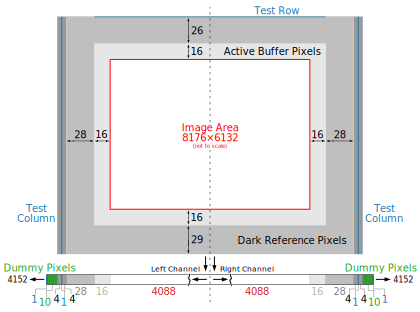
\includegraphics[width=\textwidth]{images/chip}
    \end{center}
    \caption[The layout of the CCD chips in the MicroLine cameras used by GOTO]{
        The layout of the CCD chips in the MicroLine cameras used by GOTO.\@ The central image area is not shown to scale, but the surrounding rows and columns are all in proportion.
        }\label{fig:chip}
\end{figure}

\begin{figure}[p]
    \begin{center}
        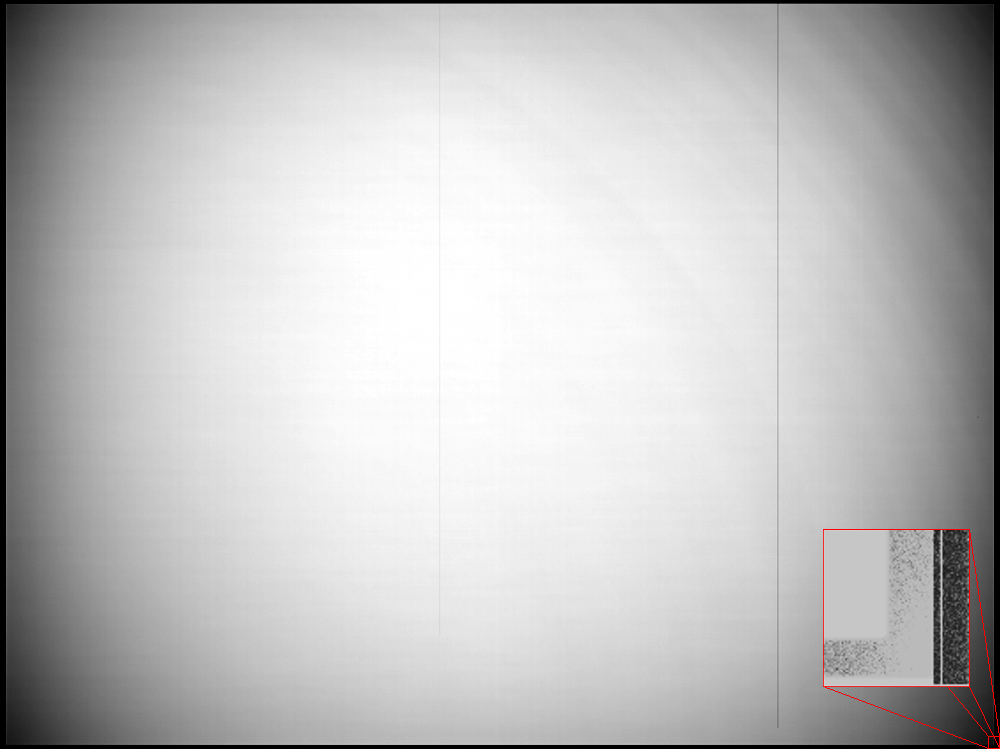
\includegraphics[width=\textwidth]{images/sample.png}
    \end{center}
    \caption[TODO]{
        A sample bright frame from one of the GOTO cameras. The highlighted area in the corner shows some of the features described in \aref{fig:chip}. Also note the two bad columns.
        }\label{fig:frame}
\end{figure}

\clearpage

\end{colsection}

% ~~~~~~~~~~~~~~~~~~~~
\subsection{In-lab tests}
\label{sec:detector_tests}
\begin{colsection}

The first of the FLI cameras to be used on GOTO arrived in Warwick in February 2016, and in March it was moved to Sheffield to carry out a detailed study.
The first camera was bought up to Sheffield on 8th March with a collection of other hardware, it was taken back when the other three were delivered on 10th May. These cameras were returned to Warwick on 8th June.

The results of the analysis were written up as a page on the GOTO wiki for easy access and reference, and are repeated below.

\begin{table}[t]
    \begin{center}
        \begin{tabular}{cccc} %chktex 44
            Name     & Serial number & Set & Tested     \\
            \midrule
            Camera 1 & ML0010316     & 1   & June---??? 2016 \\
            Camera 2 & ML0330316     & 1   & April---June 2016 \\
            Camera 3 & ML0420516     & 1   & June--??? 2016 \\
            Camera 4 & ML0430516     & 1   & June--??? 2016 \\
            \\
            Camera 5 & ML5644917     & 2   & May---June 2018 \\
            Camera 6 & ML6054917     & 2   & May---June 2018 \\
            Camera 7 & ML6094917     & 2   & May---June 2018 \\
            Camera 8 & ML6304917     & 2   & May---June 2018 \\
            \\
            Camera 9 & ML6314917     & --- & --- \\
        \end{tabular}
    \end{center}
    \caption[List of GOTO cameras]{
        A list of the 9 GOTO cameras, with assigned names, serial numbers and when they were tested.
        }\label{tab:cameras}
\end{table}


% ---------
\newpage
\subsubsection{Bias}

\begin{table}[t]
    \begin{center}
        \begin{tabular}{c|rr|rr} %chktex 44
             & \multicolumn{2}{c|}{Sheffield} & \multicolumn{2}{c}{FLI} \\
             & \multicolumn{1}{c}{L} &
               \multicolumn{1}{c|}{R} &
               \multicolumn{1}{c}{L} &
               \multicolumn{1}{c}{R} \\
            \midrule
            Camera 1 &  $971\pm4$ &  $969\pm4$ & $970.6$ &  $965.6$ \\
            Camera 2 &  $989\pm3$ &  $989\pm3$ & $995.7$ &  $988.7$ \\
            Camera 3 & $1004\pm3$ &  $991\pm3$ & $995.6$ &  $989.0$ \\
            Camera 4 &  $974\pm3$ & $1008\pm4$ & $969.7$ & $1000.6$ \\
            Camera 5 &  $994\pm3$ &  $986\pm3$ & $989.8$ &  $978.7$ \\
            Camera 6 &  $984\pm3$ &  $991\pm3$ & $968.1$ &  $976.8$ \\
            Camera 7 &  $992\pm3$ &  $981\pm3$ & $984.2$ &  $975.6$ \\
            Camera 8 & $1008\pm3$ & $1012\pm3$ & $995.5$ &  $996.9$ \\
        \end{tabular}
    \end{center}
    \caption[TODO]{
        Bias levels (in ADU) measured in Sheffield and from the FLI test sheets.
        }\label{tab:bias}
\end{table}

\begin{table}[t]
    \begin{center}
        \begin{tabular}{c|rr|rr|rr} %chktex 44
            &
            \multicolumn{2}{c|}{1$\times$1 binning} &
            \multicolumn{2}{c|}{2$\times$2 binning} &
            \multicolumn{2}{c}{3$\times$3 binning}
            \\
             &
            \multicolumn{1}{c}{L} &
            \multicolumn{1}{c|}{R} &
            \multicolumn{1}{c}{L} &
            \multicolumn{1}{c|}{R} &
            \multicolumn{1}{c}{L} &
            \multicolumn{1}{c}{R}
            \\
            \midrule
            Camera 1 &  $971\pm4$ &  $969\pm4$ & $1036\pm5$ & $1022\pm5$ & $1145\pm7$ & $1127\pm6$\\
            Camera 2 &  $989\pm3$ &  $989\pm3$ & $1045\pm4$ & $1038\pm4$ & $1152\pm6$ & $1143\pm6$\\
            Camera 3 & $1004\pm3$ &  $991\pm3$ & $1060\pm4$ & $1054\pm4$ & $1153\pm5$ & $1149\pm5$\\
            Camera 4 &  $974\pm3$ & $1008\pm4$ & $1031\pm4$ & $1063\pm4$ & $1122\pm5$ & $1155\pm6$\\
        \end{tabular}
    \end{center}
    \caption[TODO]{
        Bias levels (in ADU) for different binning factors.
        }\label{tab:bias_bins}
\end{table}

% REMOVE FLI
% Masters are the average of 50 0-s frames
% Then take median of statistics region, in the centre of the frame
% I'm going to have to talk about overscan I fear

For a standard full-frame image there are two methods to correct for bias: using the overscan regions and using a master bias.

The two 10-pixel wide dummy regions on either side of the image as shown in \aref{fig:chip} can be subtracted from the frame (independently for each channel) to correct for much of the bias level. These levels change for each image, but typical values for each camera and channel are given in \aref{tab:bias} --- they are usually between 960 and 990 counts.

For each camera 50 dark, zero-exposure full-frame images were taken, overscan subtracted and stacked in order to construct a master bias frame. This can be used to correct for any structure in the bias level. The most obvious structure is a difference in bias levels between the two channels in each camera. The average remaining field bias values are also listed in \aref{tab:bias}.

% ---------
\newpage
\subsubsection{Sources of noise}

There are multiple sources of noise in images taken with CCD cameras \citep{CCDs}:

\begin{itemize}
    \item Shot noise from the source object ($\sigma_\text{O}$), due to photons arriving at different times. When carrying out on-sky astronomical observations the source noise is typically divided into noise from the target object and noise from the background sky, but this is not relevant for the in-lab tests described in this section.

    \item Dark current noise ($\sigma_\text{DC}$), shot noise from thermally generated electrons within the CCD chip. The electrons produced by thermal excitations are indistinguishable from photo-electrons, and will increase with exposure time. Cooling the cameras will reduce the dark current.

    \item Read-out noise ($\sigma_\text{RO}$) from the camera electronics. The read-out noise depends on the speed data is read out from the CCD, the FLI MicroLine cameras ead out at a fixed \SI{8}{\mega\hertz} but some astronomical cameras have variable read-out speeds. As a property of the output electronics the read-out noise is independent of signal or the exposure time used, and each of the two channels in the camera will have an independent read-out noise.

    \item Fixed-pattern noise ($\sigma_\text{FP}$) from different sensitivities between pixels, also known as the \gls{prnu}. This noise is a physical aspect of each pixel and so remains constant between images like bias, but unlike bias it will increase linearly with the input signal. It is usually described as a percentage of the full-well capacity.

\end{itemize}

The values described above are all independent Gaussian random variables, and therefore they are added in quadrature to get the total noise

\begin{equation}
    \sigma^2 = \sigma_\text{O}^2 + \sigma_\text{DC}^2 + \sigma_\text{RO}^2 + \sigma_\text{FP}^2.
    \label{eq:noise}
\end{equation}

% ---------
\newpage
\subsubsection{Photon transfer curves}

% https://harvestimaging.com/blog/?p=1034
% https://www.couriertronics.com/docs/notes/cameras_application_notes/Photon_Transfer_Curve_Derivation.pdf
% http://slittlefair.staff.shef.ac.uk/teaching/phy217/lectures/instruments/L14/index.html
% https://www-spiedigitallibrary-org.sheffield.idm.oclc.org/ebooks/PM/Scientific-Charge-Coupled-Devices/eISBN-9780819480392/10.1117/3.374903

The \gls{ptc} is a method to determine the gain, read-out and fixed-pattern noise for a CCD camera \citep{PTC}. To construct a PTC a series of bright exposures of a flat light source were taken with varying exposure times. For these tests the dark current noise is negligible, so the $\sigma_\text{DC}^2$ term in \aref{eq:noise} can be ignored and the total noise in a bright image is given by

\begin{equation}
    \sigma^2 = \sigma_\text{O}^2 + \sigma_\text{RO}^2 + \sigma_\text{FP}^2.
    \label{eq:ptc_noise1}
\end{equation}

These noise values are given in electrons (\elec), but what we record in our image files is the signal ($S$) in ADU.\ This signal is linearly related to the actual number of electrons detected ($N$) through the gain ($g$), in \elec/ADU, as

\begin{equation}
    N = g S.
    \label{eq:gain}
\end{equation}

The gain is an important parameter of a CCD, which can be set to best utilise the dynamic range of the detector. The KAF-50100 detectors have a specification full well capacity of 40,300 electrons before they saturate, and the cameras have a 16-bit readout (meaning the signal from each pixel can vary from 0 to 65535 ($2^{16}$) ADU). Therefore if the gain is set to $1$ \elec/ADU a saturated pixel would produce a signal of 40300 ADU, which is only using two-thirds of the dynamic range.

Since \aref{eq:gain} shows the signal $S$ is directly proportional to the number of electrons $N$, their errors are also directly proportional with the same constant. Therefore error measured in the signal, $\sigma_S$, is related to the error in the electron count as

\begin{equation}
    \sigma_N = g \sigma_S.
    \label{eq:noise_gain}
\end{equation}

The shot noise from the source object comes from counting photo-electrons, and the arrival time of the photons is a Poisson distribution (this is also true for the thermal electrons producing dark current). If the number of electrons counted is $N$, for large $N$ this tends towards a Gaussian distribution with mean $N$ and standard deviation

\begin{equation}
    \sigma_N = \sqrt{N}.
    \label{eq:shot_noise}
\end{equation}

As described previously the read-out noise is a fixed property of the CCD electronics, and therefore does not vary between pixels or exposures. The fixed-pattern noise also comes from a physical aspect of the detector: the small differences in size and response between pixels known as the \glsfirst{prnu}. This noise is proportional to the number of electrons detected, so can be written as

\begin{equation}
    \sigma_\text{FP} = k_\text{FP}N = k_\text{FP}gS,
    \label{eq:fp_noise}
\end{equation}

where $k_\text{FP}$ is a dimensionless constant of proportionality describing the fixed-pattern noise, and is given in percent. Scientific CCD cameras typically have very small PRNUs, of the order of $<1\%$.

Adding the above noise terms into \aref{eq:ptc_noise1} gives

\begin{equation}
    g^2\sigma_S^2 = g S + \sigma_\text{RO}^2 + k_{FP}^2 g^2 S^2,
    \label{eq:ptc_noise2}
\end{equation}

which can be written in the form

\begin{equation}
    \sigma_S^2 = {\left(\frac{\sigma_\text{RO}}{g}\right)}^2 +
                 \frac{1}{g}S +
                 k_\text{FP}^2 S^2.
    \label{eq:ptc}
\end{equation}

This is a quadratic equation relating the measured signal $S$ to the variance in the signal $\sigma_S^2$, where $S$ and $\sigma_S$ are in ADU, $\sigma_\text{RO}$ is in \elec, $g$ is in \elec/ADU and $k_\text{FP}$ is dimensionless.

A \glsfirst{ptc} is a log-log plot of signal $S$ vs standard deviation $\sigma$, and by fitting \aref{eq:ptc} to this data values for the gain, read-out noise and fixed-pattern noise can be determined. The key features of a photon transfer curve are common for all CCDs, and are shown in cartoon form in \aref{fig:ptc_cartoon}.
.
\newpage

\begin{figure}[t]
    \begin{center}
        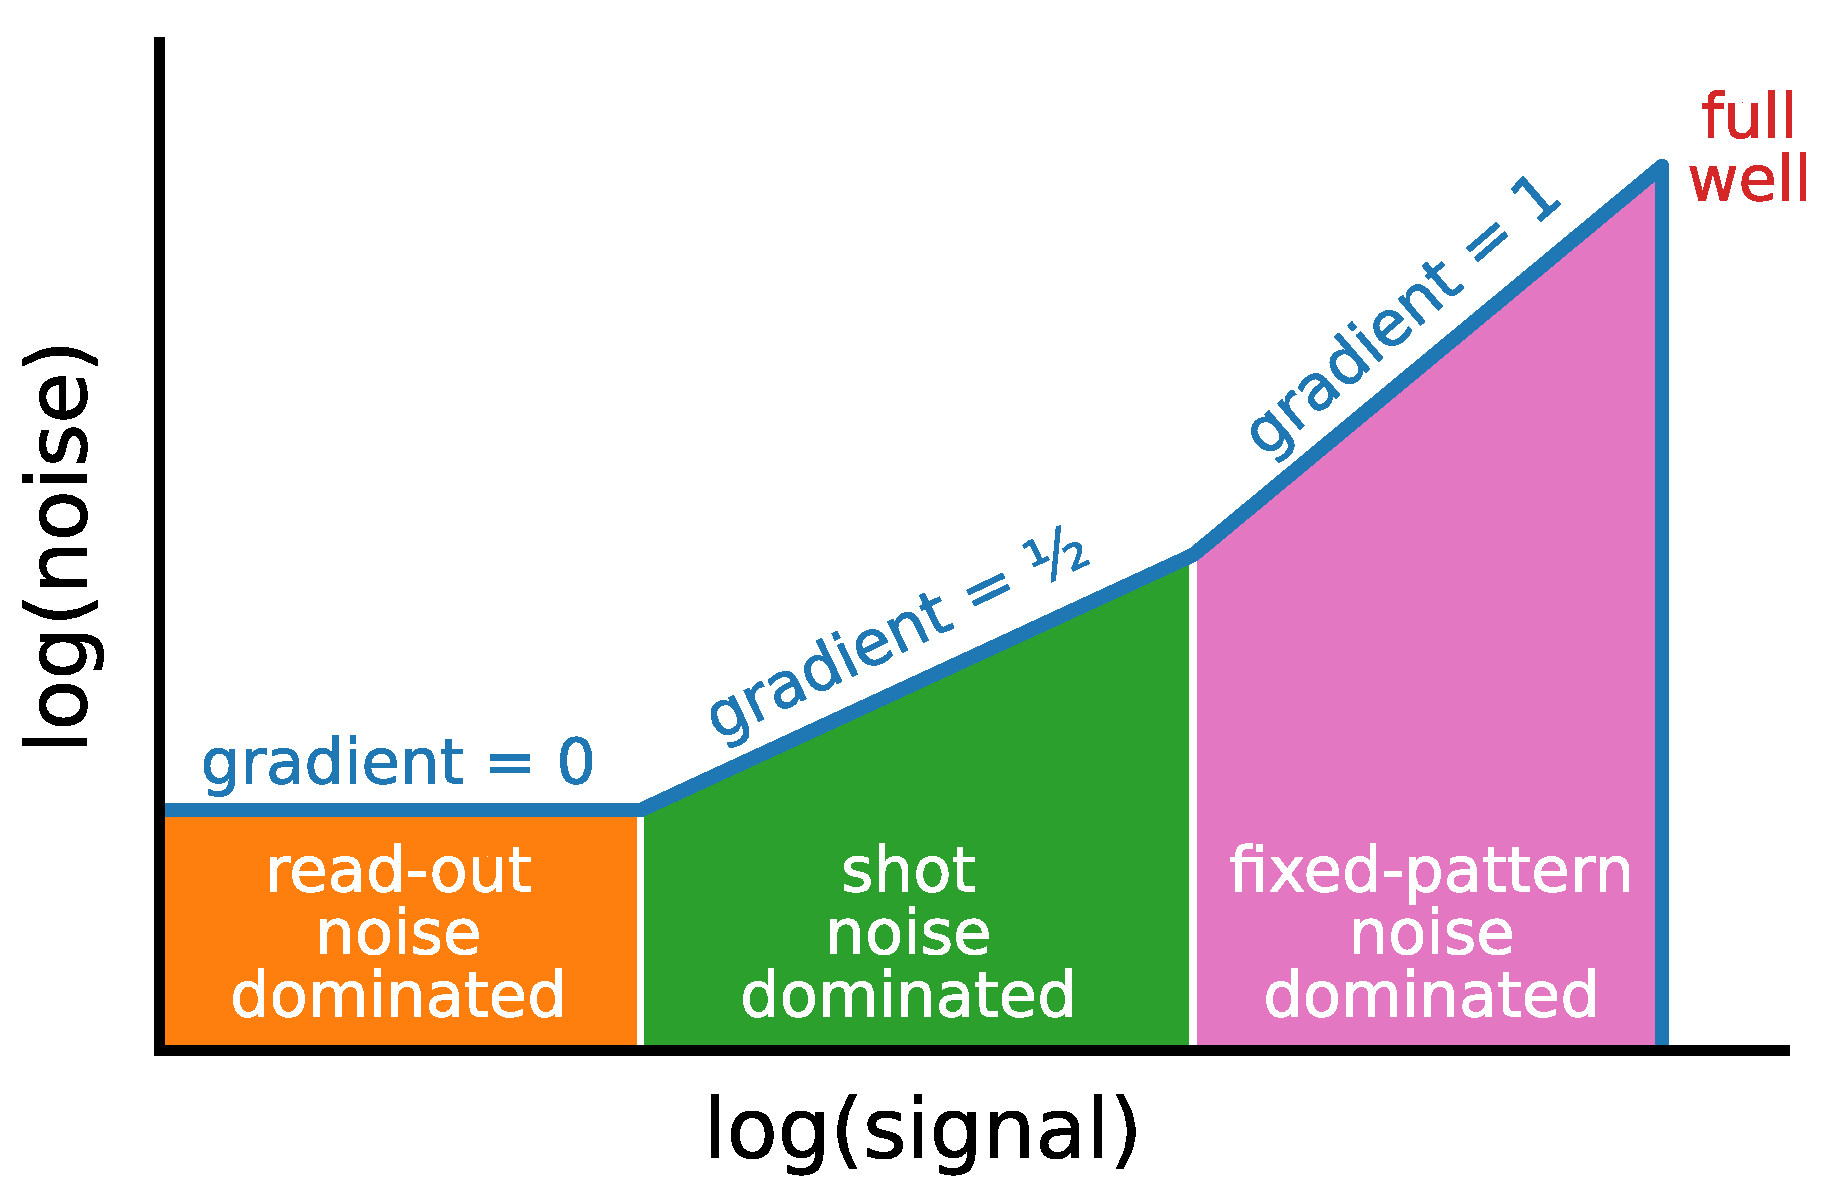
\includegraphics[width=0.65\textwidth]{images/ptc.pdf}
    \end{center}
    \caption[Key features of the photon transfer curve]{
        The key features of a photon transfer curve, adapted from Figure 2.2 of \citet{CCDs}.
        }\label{fig:ptc_cartoon}
\end{figure}

There are three visible noise regimes in the photon transfer curve. The first is when the signal is zero. For small $S$ in \aref{eq:ptc} the noise is constant, and as there is no signal the overall noise is limited by the detector noise. This will include both the read-out noise and the dark current, but as these are very short exposure times (less than 1 second) the dark current is completely negligible and the read-out noise dominates. At higher signals the noise is dominated by the shot noise. As this is proportional to the square root of the signal this region has a gradient of 1/2 when plotted on the log-log axis, and when $\sigma_S$ is zero the signal will equal the gain (i.e.\ the value of the gain is where the linear fit crosses the x-axis). As the signal increases further the fixed-pattern noise begins to dominate over the shot noise, as it is proportional to the signal this produces a gradient of 1 in the \gls{ptc}. Finally the pixel will reach its full well value and saturate, so the noise drops to zero.

As it is impossible to know the exact number of incoming photons on each pixel, it is not possible to determine the signal and noise values for a given pixel. Instead the PTC is constructed by selecting a region of pixels and plotting the mean signal value against the standard deviation. Repeated for several regions across the image this gives a reasonable approximation of the average noise in each pixel.

\newpage

\begin{table}[t]
    \begin{center}
        \begin{tabular}{l|cc|cc|cc} %chktex 44
             &
            \multicolumn{2}{c|}{Gain} &
            \multicolumn{2}{c|}{RO noise} &
            \multicolumn{2}{c}{FP noise} \\
            &
            \multicolumn{2}{c|}{(\elec/ADU)} &
            \multicolumn{2}{c|}{(\elec)} &
            \multicolumn{2}{c}{(\%)} \\
             & L & R & L & R & L & R \\
            \midrule
            Camera 1 & 0.53 & 0.53 & 12.4 & 12.0 & 0.46 & 0.45 \\
            Camera 2 & 0.53 & 0.53 & 11.9 & 11.7 & 0.44 & 0.46 \\
            Camera 3 & 0.57 & 0.57 & 12.6 & 11.8 & 0.45 & 0.42 \\
            Camera 4 & 0.57 & 0.58 & 13.4 & 14.0 & 0.41 & 0.43 \\
            Camera 5 & 0.62 & 0.63 & 12.3 & 12.8 & 0.40 & 0.40 \\
            Camera 6 & 0.63 & 0.62 & 11.8 & 12.6 & 0.40 & 0.40 \\
            Camera 7 & 0.62 & 0.62 & 13.1 & 12.5 & 0.41 & 0.39 \\
            Camera 8 & 0.62 & 0.62 & 14.3 & 12.2 & 0.41 & 0.39 \\
        \end{tabular}
    \end{center}
    \caption[TODO]{
        Results of fitting photon transfer curves for each of the eight cameras.
        }\label{tab:ptc}
\end{table}

\glspl{ptc} were constructed for all eight cameras, by taking flat images of varying exposure times. Twelve 50$\times$50 pixel regions were selected across the field, and the mean and standard deviation of the pixel values were plotted to form the \gls{ptc}. These are shown in \aref{fig:ptcs}. The curves were fitted to \aref{eq:ptc}, and the resulting values for the gain, read-out noise and fixed-pattern noise are given in \aref{tab:ptc}.

As expected, the gain values are all around 0.6 \elec/ADU, and would have been set as such to maximise the dynamic range. There is a clear difference in gain levels between the first set of cameras (1--4) and the second set (5--8), which is most likely due to changes made by FLI over the two years between their manufacture. The read-out noise values are all around 11--14 \elec, and match the FLI specifications which advertise a typical system noise of 12 \elec{} when reading out at \SI{8}{\mega\hertz}. The two channels on each camera are independent and therefore there is no correlation in read-out noise, unlike the gain which is always approximately the same in each amplifier. Finally the fixed-pattern noise is always below 0.5\% of the signal as expected. The fraction notably decreases from $\sim$0.45\% to $\sim$0.40\%; if this is related to improved chip manufacturing this might explain the reason FLI were able to set the gain higher for the later cameras. However, this test only includes a small sample of the 50 million pixels on each chip, and so might not be a perfect measure of the overall photo response non-uniformity.

\begin{figure}[p]
    \begin{center}
        \begin{minipage}[t]{0.49\textwidth}\vspace{10pt}
            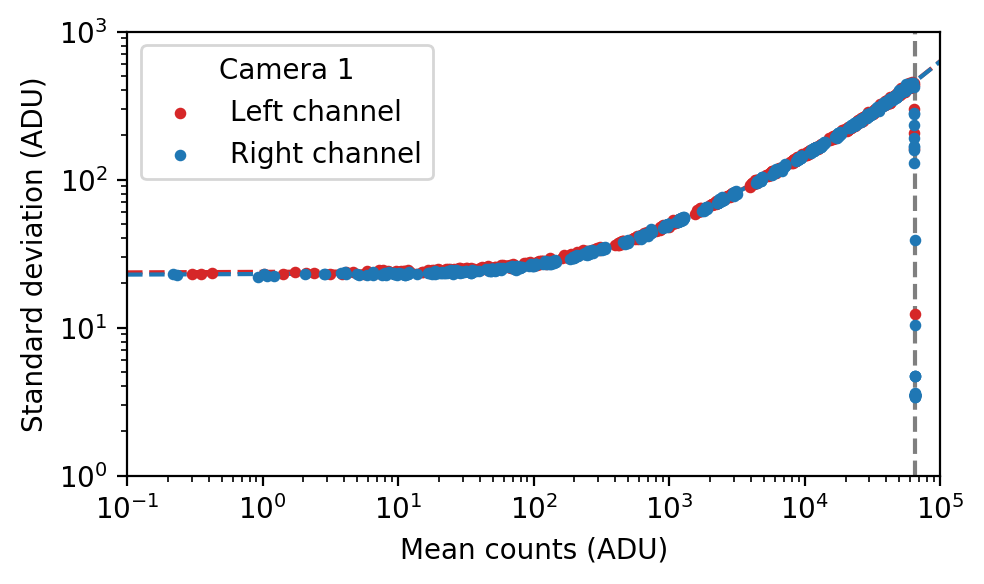
\includegraphics[width=\linewidth]{images/detectors/ptc_1.png}
        \end{minipage}
        \begin{minipage}[t]{0.49\textwidth}\vspace{10pt}
            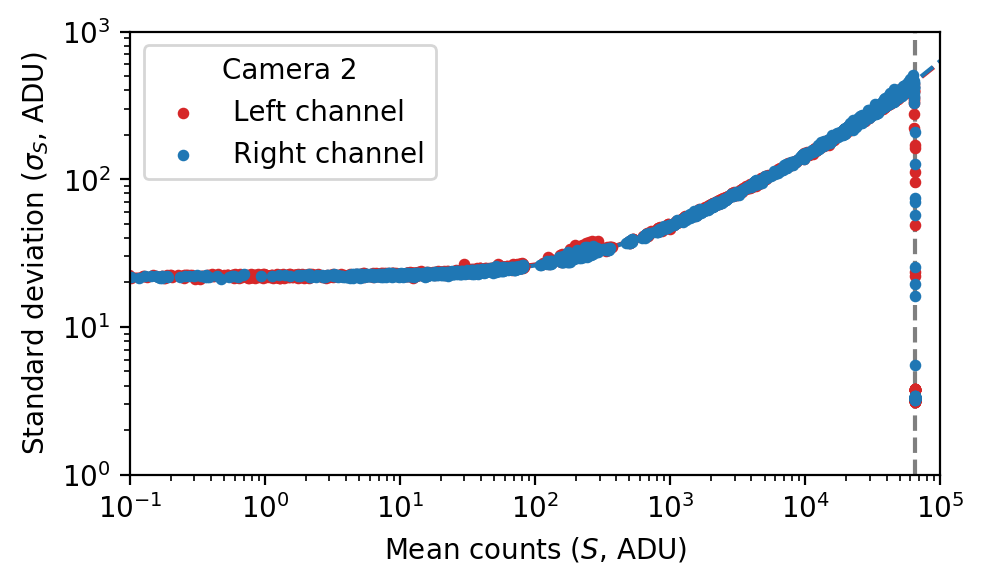
\includegraphics[width=\linewidth]{images/detectors/ptc_2.png}
        \end{minipage}

        \begin{minipage}[t]{0.49\textwidth}\vspace{10pt}
            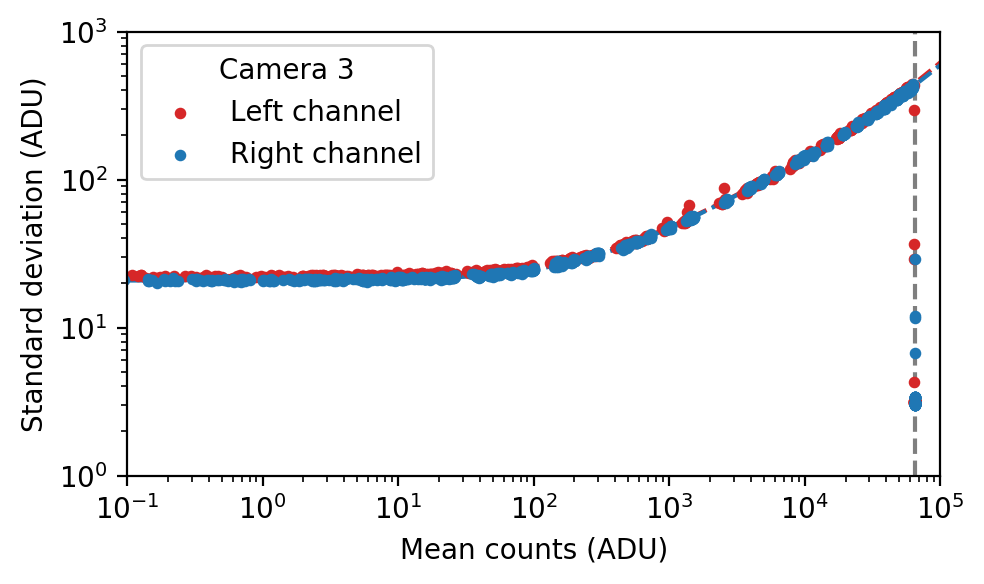
\includegraphics[width=\linewidth]{images/detectors/ptc_3.png}
        \end{minipage}
        \begin{minipage}[t]{0.49\textwidth}\vspace{10pt}
            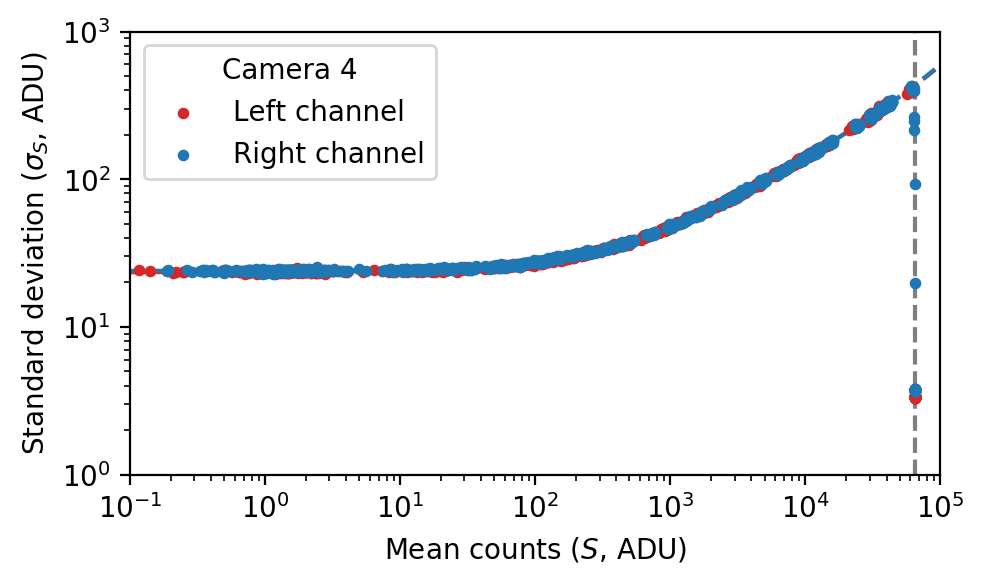
\includegraphics[width=\linewidth]{images/detectors/ptc_4.png}
        \end{minipage}

        \begin{minipage}[t]{0.49\textwidth}\vspace{10pt}
            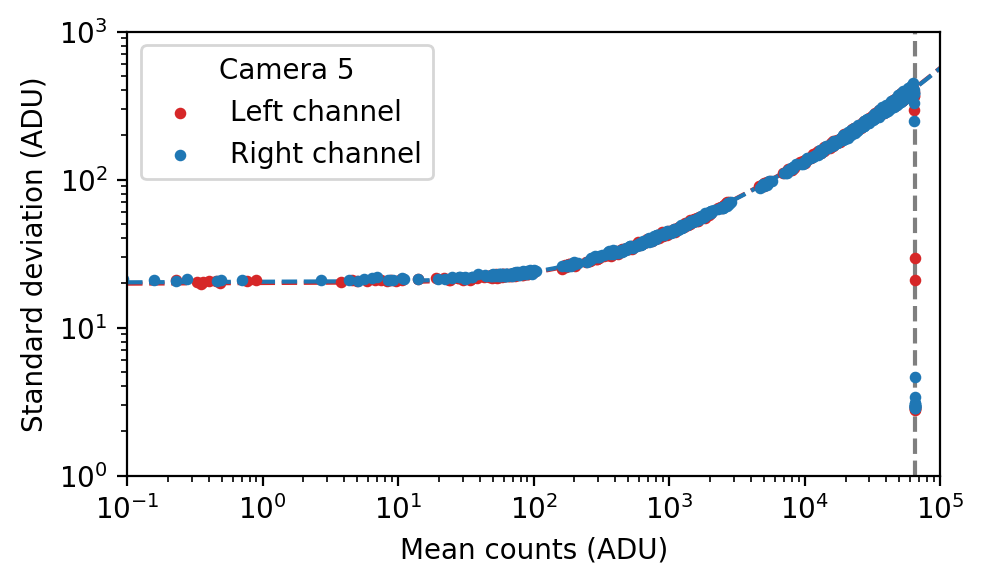
\includegraphics[width=\linewidth]{images/detectors/ptc_5.png}
        \end{minipage}
        \begin{minipage}[t]{0.49\textwidth}\vspace{10pt}
            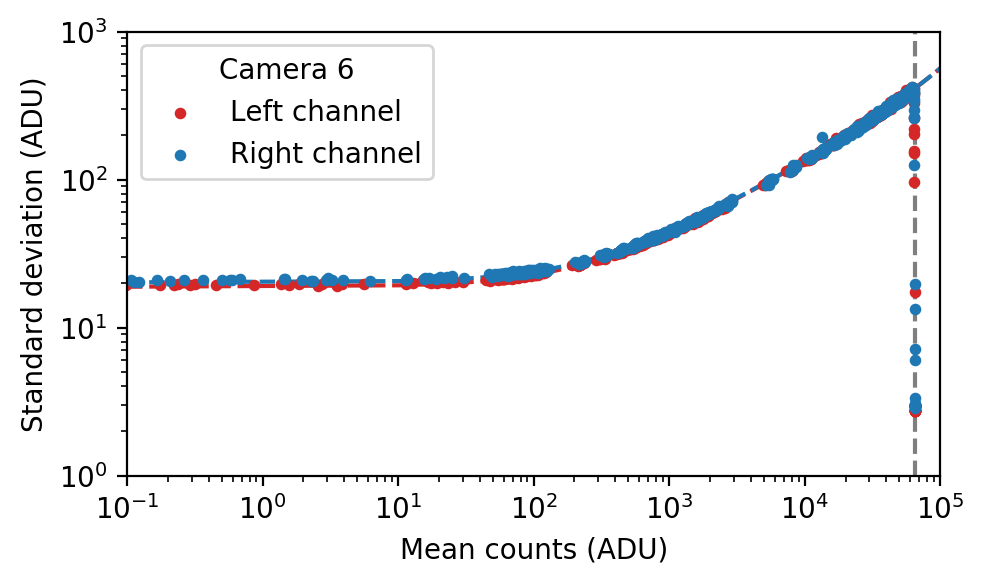
\includegraphics[width=\linewidth]{images/detectors/ptc_6.png}
        \end{minipage}

        \begin{minipage}[t]{0.49\textwidth}\vspace{10pt}
            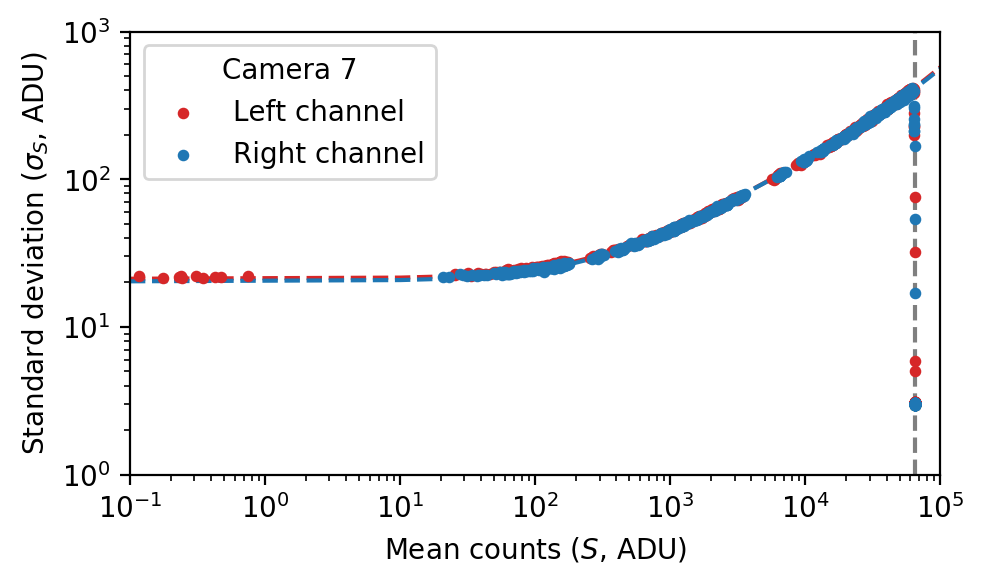
\includegraphics[width=\linewidth]{images/detectors/ptc_7.png}
        \end{minipage}
        \begin{minipage}[t]{0.49\textwidth}\vspace{10pt}
            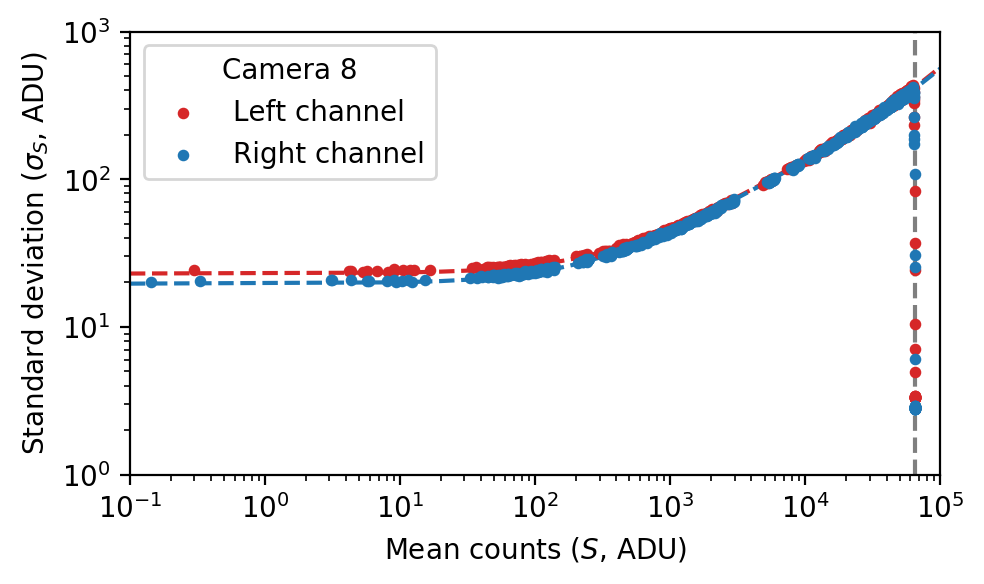
\includegraphics[width=\linewidth]{images/detectors/ptc_8.png}
        \end{minipage}
    \end{center}
    \caption[Photon transfer curves for all 8 cameras]{
        Photon transfer curves for all 8 cameras.
        }\label{fig:ptcs}
\end{figure}

\clearpage

% ---------
\newpage
\subsubsection{Dark current}

\begin{table}[t]
    \begin{center}
        \begin{tabular}{c|rr} %chktex 44
            % & \multicolumn{2}{c}{Sheffield} \\
             & \multicolumn{1}{c}{L} & \multicolumn{1}{c}{R} \\
            \midrule
            Camera 1 & $0.0022\pm0.0014$ & $0.0017\pm0.0014$ \\
            Camera 2 & $0.0030\pm0.0014$ & $0.0027\pm0.0013$ \\
            Camera 3 & $0.0034\pm0.0013$ & $0.0036\pm0.0012$ \\
            Camera 4 & $0.0026\pm0.0014$ & $0.0030\pm0.0014$ \\
            Camera 5 & $0.0015\pm0.0012$ & $0.0017\pm0.0013$ \\
            Camera 6 & $0.0020\pm0.0012$ & $0.0017\pm0.0013$ \\
            Camera 7 & $0.0017\pm0.0013$ & $0.0014\pm0.0013$ \\
            Camera 8 & $0.0019\pm0.0014$ & $0.0015\pm0.0013$ \\
        \end{tabular}
    \end{center}
    \caption[TODO]{
        Dark current (in ADU/sec) measured at \SI{-25}{\celsius}.
        }\label{tab:dark}
\end{table}

\citep{dark_current}

Dark current was analysed as a function of temperature. This required long (30 minute) dark exposures, taken overnight to reduce background light. Each camera produced a clear exponential trend, a curve was fitted defined by the dark current at -25°C (an arbitrary point, but matched to the spec definition) and the dark current doubling temperature. The results are shown in \aref{tab:dark}.

The preliminary specification sheet gave a typical value of 0.002 electrons/pixel/second for the dark current at -25°C, all the cameras were around this value although with some deviation. The revised spec gave an expected value of 0.008 e-/pix/sec, well above what we measure.

The dark current was also examined as a function of time since power on, as in some cameras (such as ULTRASPEC) the dark current reduces slowly. No such trend was visible using the FLI cameras. However since the detector and cooler are integrated into the same body there has to be some time spent waiting after power on for the camera to cool to the target temperature, thus negating the effect.

% ---------
\newpage
\subsubsection{Linearity}

Linearity was measured for all four cameras using a flat light source and increasing exposure times. Each camera had a turn off in the lower half of the dynamic range which needs further analysis, this experiment was hampered by the broken flat light source. Very short exposure times were studied in order to see any possible effect of the shutter speed. It was found that although the cameras allow exposure times as low as 1ms there is a consistent deviation from linearity below approximately 0.15 seconds. As such exposure times shorter than 0.2 seconds should be avoided.

% ---------
\newpage
\subsubsection{Timing}

An analysis was carried out attempting to measure the readout speeds of the CCD, and thus the minimum dead time required for a given frame. However, as the cameras do not have enough memory to store an entire frame (communication with FLI) readout must begin immediately after the exposure has finished in order to prevent the data being overwritten. This typically takes approximately 3 seconds for a full frame.

% ---------
\newpage
\subsubsection{Defects}

\begin{table}[t]
    \begin{center}
        \begin{tabular}{cc|lll} %chktex 44
            Camera   & Serial    & \multicolumn{3}{c}{Dark Columns} \\
            \midrule
            Camera 1 & ML0010316 & 1 dead column:  & x=7678, starting at y=4312 & (30\%) \\
            Camera 2 & ML0330316 & 2 dead columns: & x=3583, starting at y=909  & (85\%) \\
                     &           &                 & x=6386, starting at y=127  & (98\%) \\
            Camera 3 & ML0420516 & 2 dead columns: & x=1800, starting at y=1151 & (81\%) \\
                     &           &                 & x=5140, starting at y=4986 & (19\%) \\
            Camera 4 & ML0430516 & 1 dead column:  & x=5333, starting at y=2561 & (58\%) \\
        \end{tabular}
    \end{center}
    \caption[TODO]{
        Locations of dead columns caused by stuck pixels. The percentages denote the amount of the column that is unusable.
    }\label{tab:frame}
\end{table}

For each camera a defect mask was constructed using the ratio of two flat images of different exposures, and then detecting pixels outside of a given sigma limit. Each camera was found to have at least one stuck pixel, which produced a dead column travelling up the frame. In \aref{fig:frame} these are visible as two dark columns. The exact positions and details for every camera are shown in \aref{tab:frame}.

The ONSemi chip specifications gives an allowed limit of less than 20 column defects per device, and none of the GOTO detectors had more than two.

% ---------
\newpage
\subsubsection{Results}

Overall the initial characterization of the detectors managed to agree with the specifications provided by FLI.\@ In the case of the critical PTC values (gain, noise etc\ldots) FLI carried out their own analysis which I only received the results of after my own analysis had finished. These are given in \aref{tab:ptc} and show very similar results to the ones observed in Sheffield. More complete characterization will be possible once the telescope is up an running, in particular using the sky for flat-field and point-source tests which were limited by the equipment available here.

\end{colsection}

% ~~~~~~~~~~~~~~~~~~~~
\newpage
\subsection{Throughput modelling}
\label{sec:throughput}
\begin{colsection}

WIP

\end{colsection}

% ~~~~~~~~~~~~~~~~~~~~

\end{colsection}

% ########################################

\newpage
\section{Deploying the hardware}
\label{sec:hardware}
\begin{colsection}

% ~~~~~~~~~~~~~~~~~~~~

\begin{colsection}

WIP

\end{colsection}

% ~~~~~~~~~~~~~~~~~~~~

\subsection{Construction on La Palma}
\label{sec:construction}
\begin{colsection}

WIP

\end{colsection}

% ~~~~~~~~~~~~~~~~~~~~

\subsection{Extra dome systems}
\label{sec:arduino}
\begin{colsection}

WIP

\end{colsection}

% ~~~~~~~~~~~~~~~~~~~~

\end{colsection}

% ########################################

\newpage
\section{Developing observing routines}
\label{sec:obs_scripts}
\begin{colsection}

% ~~~~~~~~~~~~~~~~~~~~

\begin{colsection}

WIP

\end{colsection}

% ~~~~~~~~~~~~~~~~~~~~

\subsection{Taking flat fields}
\label{sec:flats}
\begin{colsection}

WIP \citep{flats}

\end{colsection}

% ~~~~~~~~~~~~~~~~~~~~

\subsection{Focusing the telescopes}
\label{sec:autofocus}
\begin{colsection}

WIP \citep{autofocus}

\end{colsection}

% ~~~~~~~~~~~~~~~~~~~~

\end{colsection}

% ########################################

\newpage
\section{Observing results}
\label{sec:observing}
\begin{colsection}

% ~~~~~~~~~~~~~~~~~~~~

\begin{colsection}

WIP

\end{colsection}

% ~~~~~~~~~~~~~~~~~~~~

\subsection{The all-sky survey}
\label{sec:survey_results}
\begin{colsection}

WIP

\end{colsection}

% ~~~~~~~~~~~~~~~~~~~~

\subsection{Gravitational wave observations}
\label{sec:gw_results}
\begin{colsection}

WIP

\end{colsection}

% ~~~~~~~~~~~~~~~~~~~~

\subsection{Other transient follow-up}
\label{sec:other_results}
\begin{colsection}

WIP

\end{colsection}

% ~~~~~~~~~~~~~~~~~~~~

\end{colsection}

% ########################################
